\newpage
\section{Experimentos}

	En el presente capítulo se abordan las diferentes etapas que engloban a los experimentos de esta tesis. En las primeras 2 secciones se describen tanto las métricas y protocolos de evaluación utilizados en el dataset como así también los conjuntos de entrenamiento que se utilizan en los experimentos. Posteriormente, se detallan los parámetros que se utilizan en los diferentes experimentos y los resultados obtenidos de los mismos. Por último, se brinda un análisis de los resultados con el fin de evaluar la eficiencia del clasificador en las diferentes pruebas.

	\subsection{Métricas y Protocolo de Evaluación}

\FL{Explicar cómo se divide el dataset en train y test y qué métricas se calculan sobre el test (accuracy por ejemplo).}
	
	
	\subsection{Conjuntos de Entrenamiento}

	En esta sección se va a discutir los diferentes conjuntos de entrenamientos usados en los experimentos. En las evaluaciones se trabaja básicamente con 3 conjuntos.
	
	El primero, es el compuesto sólo por imágenes de caracteres segmentados de escenas naturales.
	
	El segundo conjunto es el armado con imágenes sintéticas, cuyo proceso de creación fue explicado en detalle en la sección \ref{subsection:impl_propia}. El grupo de imágenes de fuentes que se usa para crear los caracteres sintéticos fue extraído del dataset mencionado anteriormente en \ref{subsection:evaluacion} y consiste en 1000 imágenes por clase. De este conjunto se crearon 6 variaciones diferentes, con el objetivo de observar el impacto que tiene la cantidad de caracteres sintéticos al momento de clasificar imágenes de caracteres naturales. La cantidad de muestras por clase (variaciones) en cada conjunto de entrenamiento es el siguiente:
	\begin{itemize}
		\item Muestras por clase : $ mpc \in \{ 50,100,250,500,1000,2000\}$
	\end{itemize}

	El tercer tipo está compuesto por una combinación de los dos primeros conjuntos. Se creó con la finalidad de observar el impacto en la clasificación de integrar en diferentes proporciones imágenes sintéticas y reales al conjunto de entrenamiento. Dada la escasa cantidad de imágenes naturales para el entrenamiento (15 en total por cada clase) se busca complementar esto integrando datos sintéticos. Por consiguiente se decide crear 9 conjuntos de entrenamiento donde en cada uno se incorporan diferentes proporciones de imágenes sintéticas a las 15 reales que existentes. La proporción de cada conjunto de entrenamiento es de la siguiente manera: 
	
	$$(15, x) x \in \{0,3,8,15,30,75,150,300,750,1500 \}$$
	
	El primer elemento de la tupla $(15, x)$ corresponde a la cantidad de imágenes reales, cuyo valor es fijo. El segundo elemento de la tupla hace referencia a la proporción de caracteres sintéticos. Es fácil observar que a medida que aumentamos la proporción, la cantidad de caracteres naturales se va volviendo cada vez más despreciable. El hecho de no considerar imágenes sintéticas inicialmente $(15,0)$ tiene como finalidad el observar el cambio que se produce desde el inicio cuando no hay caracteres sintéticos en el entrenamiento. Los resultados se analizan en la última sección del presente capítulo.
	
	
	
	\subsection{Diseño de los experimentos}

	\begin{itemize}
		\item Aca debería ir una descripción de los parámetros a usar en los experimentos con una explicación de lo que se espera obtener.
		\begin{itemize}
			\item Explicar para qué sirve cada parámetro
			\item Explicar los valores que se van a usar para cada parámetro
		\end{itemize}
	\end{itemize}

	Dada la gran cantidad de parámetros que hay en el sistema, la cantidad de experimentos para encontrar la mejor configuración es extensa.

        \paragraph{Generación de datos sintéticos}

	El primer parámetro a considerar es el tipo de conjunto de entrenamiento a evaluar, como se procederá a explicar en la próxima sección, tenemos un total de 20 conjuntos diferentes. Esto con el objetivo de evaluar la performance del clasificador en diferentes ámbitos. Los parámetros utilizados durante la creación de las imágenes sintéticas son, como se explicó en el capítulo anterior, escala, rotación, blur, ruido gaussiano e inclinación. Dado que hay un abanico bastante grande valores para asignarles a estas transformaciones, se decidió por asignarle a cada una un rango de valores los cuales si bien modificaban la imagen, no la hacían ilegible. Dado que los autores en \cite{wang} no especifican el rango de valores para las transformaciones afines que utilizan, se procedió a establecer el siguiente conjunto de rangos para todas las tranformaciones utilizadas:
	
	\begin{itemize}
		\item Inclinación: factor de inclinación $n \in [-0.20 ; 0.20]$
		\item Suavizado gaussiano (blur): $\sigma \in [0 ; 2]$
		\item Escala: es igual en ambos ejes $x=y \in [0.8; 1.25]$
		\item Rotación: en radianes $\theta \in (-0.1; 0.1)$
		\item Ruido gaussiano: $\sigma \in [1; 30]$
	\end{itemize}
	
	El hecho de no contar con una replica exacta del conjunto de datos sintéticos usados por Wang et al., los conjuntos generados con estos valores claramente van a ser distintos a los originales y por ende la comparación de resultados  en \ref{subsection:resultados} va a estar influida por la forma en que se generaron los conjuntos.
	
	\paragraph{Extracción de características con HOG}

	Posteriormente tenemos los parámetros propios que utiliza HOG para extraer las características de cada imagen. HOG hace uso de dos parámetros, la cantidad de \textit{orientaciones} y la cantidad de \textit{celdas por bloque}. Como se explicó en el capítulo anterior \ref{subsection:hog}, dada una imagen, esta se dividía en regiones llamadas celdas. Dentro de cada una se realiza el calculo de las orientaciones y posteriormente dado un bloque de celdas se extraía un histograma de orientaciones de todas las celdas involucradas. Dada la gran cantidad de combinaciones entre ambos parámetros, se decidió por utilizar los siguientes valores:
	
	\begin{itemize}
		\item Orientaciones: $\{8; 9\}$
		\item Celdas por bloque: $\{4; 9\}$
	\end{itemize}
	
	La elección de estos números se debe a que reducen la tasa de errores de clasificación. Un análisis similar se puede encontrar en \cite{DT05} donde los autores (quienes crearon HOG) analizan la mejor configuración para resolver el problema de detección de personas. Si bien el problema que se busca resolver en este trabajo es totalmente diferente, los parámetros que ellos usan para HOG muestran buenos resultados en este problema también.

	\paragraph{Binarización}

	HOG devuelve descriptores de tamaño fijo dependiendo de la cantidad de orientaciones y celdas por bloque que le asignemos. Lo que buscamos con establecer una longitud variable, es evaluar la perdida o ganancia de información sobre la imagen al realizar esto y ver si hay algun impacto en la performance al final. Para poder realizar este ``estiramiento'' o ``reducción'' de los vectores, nos aprovechamos del proceso de binarización explicado anteriormente. El impacto producido al realizar esto es notable y se va a detallar al final del capítulo. Las dimensiones con las que se trabajan es otro parámetro (para los experimentos con imágenes sintéticas y mixtas). Los valores con los que trabajamos son los siguientes:

	\begin{itemize}
		\item Dimensión del vector final: $\{ 240; 480; 1080; 2040;  4080 \}$
	\end{itemize}
	
	La elección de estas dimensiones está directamente relacionada con el siguiente parámetro que es la cantidad de \textit{grupos} por vector, por lo cual estas dimensiones tienen que ser divisibles por cada uno de los grupos a evaluar
	
	Como último parámetro a destacar en la binarización, y lo consideramos como uno de los más importantes, es el método aplicado al momento de generar el umbral de binarización. Como se podrá ver en la subsección de Resultados del capítulo 4, es muy grande el impacto obtenido en la precisión final del clasificador debido a este parámetro. La elección de qué método utilizar fue libre con el objetivo de evaluar cual era el que otorgaba mejores resultados. Se trabajaron con los siguientes métodos:

	\begin{itemize}
		\item Media
		\item Mediana
		\item Bootstrap
		\item Exponencial
	\end{itemize}
	
	Dado que los autores en \cite{wang} no especifican que método usaron al momento de binarizar los vectores. Proponemos estos cuatro métodos. Al igual pasó con los parámetros para generar los datos sintéticos, en el \cite{wang} no se aclara que método se utilizó para la binarización de los vectores, con lo cual todos los resultados obtenidos en los experimentos realizados con imágenes reales y sintéticas van a ser distintos de los originales por más de que, en el caso de las imágenes reales, se usen los mismos conjuntos de entrenamiento y prueba. \RC{Discutir esto, IMPORTANTE.}
		
	\paragraph{Entrenamiento}

	En la etapa de entrenamiento, hay 2 parámetros: la cantidad de bits por \textit{grupo} que determina finalmente la cantidad de grupos en la que se divide cada vector y \textit{alpha} que es un parámetro de inicialización para las tablas. La cantidad de grupos en las que se divide un vector impacta en el tamaño de las tablas y en la clasificación posterior. La cantidad bits denotan la cantidad de dimensiones de cada grupo, por lo cual  la cantidad de grupos esta dado por la división entre la dimensión total del vector y la dimensión del grupo.

	El parámetro \textit{alpha} es necesario ya que las tablas no se pueden inicializar con el valor $0$. Esto es debido ya que, como se explico en la sección \ref{subsection:ferns}, al momento de evaluar una imagen de prueba, puede darse el caso de que se acceda a una posición de la tabla que nunca fue entrenada por lo cual la probabilidad se hace 0 y es un inconveniente para los cálculos posteriores. Los valores por encima de 1 no son convenientes para inicializar las tablas pues afectan a los resultados al momento de normalizarlas.

	\begin{itemize}
		\item Dimensión del grupo: $\{ 1; 2; 4; 8; 10; 12 \}$
		\item Alpha: $\{ 0.01; 0.1; 1 \}$
	\end{itemize}


	\newpage
\subsection{Resultados}
\label{subsection:resultados}
	tablas, gráficos, análisis y recomendaciones
	\begin{itemize}
		\item Aca debería explicar como fueron procesados los
                  resultados y que tipo de resultados se van a mostrar (ej. los
                  que tuvieron mejor y peor performance). \JS{hay que empezar a
                  poner cuales se van a mostrar y discutir}
                \item \JS{Baseline. Comparar con Wang}
		\item Resultados de dataset con imagenes reales.
		\begin{itemize}
			\item Se presentan los mejores resultados y los parámetros con los cuales se obtuvieron. Se van a presentar los gráficos de los 2 mejores resultados junto con sus matrices de confusión.
			\item Idem pero con los peores resultados obtenidos.
		\end{itemize}
		\item Idem con dataset sintéticos
		\item Idem con dataset sintéticos + reales.

	\end{itemize}
	
	Primero van a ir los resultados de Wang extraidos del paper y expuestos en una tabla. Se tiene que explicar que el resultado obtenido por Wang es el baseline para los experimentos realizados. Un vez que presente los mejores resultados obtenidos vuelvo a generar la tabla de comparacion.
	
	\begin{table}
		\centering
	    \begin{tabular}{ | l | l | l | p{5cm} |}
    			\hline
    				\textbf{Implementación} & \textbf{Score} \\ \hline
    				Wang NATIVE+FERNS & 0.54\% \\ \hline
    				Wang SINT+FERNS & 0.47\% \\
    			\hline
    		\end{tabular}	
    		\caption{Resultados obtenidos por Wang et al. en \cite{wang}}
	\end{table}

	Resultados de haber entrenado y evaluado al clasificador con imagenes reales. Básicamente busco mostrar que llegamos a resultados similares con Wang. Despues de mostrar los resultados, se puede agregar una tabla chiquita comparativa de los resultados.
	
			\begin{figure}[htbp!]
				\centering
				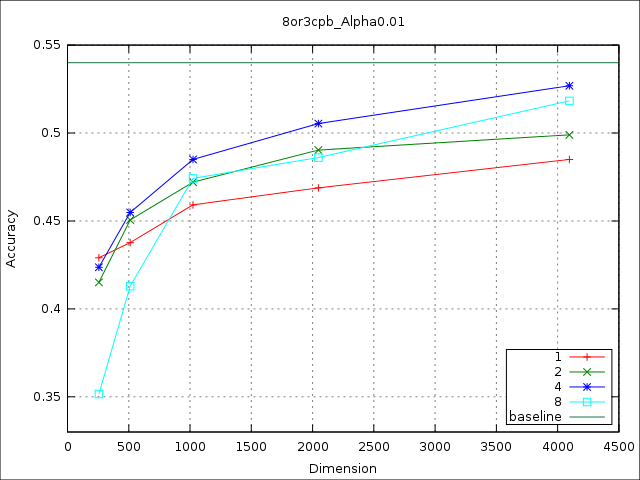
\includegraphics[scale=0.6]{img/resultados/reales/media_8or3cpb_Alpha0,01.png}
				\caption[Reales con umbral media]{Resultado de haber usado la media para el calculo del umbral. La mejor clasificación se logra con los siguientes parámetros: \textit{alpha:0.01}, \textit{bits por grupo: 4}, \textit{dim del vector: 4096}, \textit{orientaciones: 8}, \textit{celdas por bloque: 9}.}
				\label{fig: Reales-media-8or9cpbAlph0.01}
			\end{figure}
			
			\begin{figure}[htbp]
				\centering
				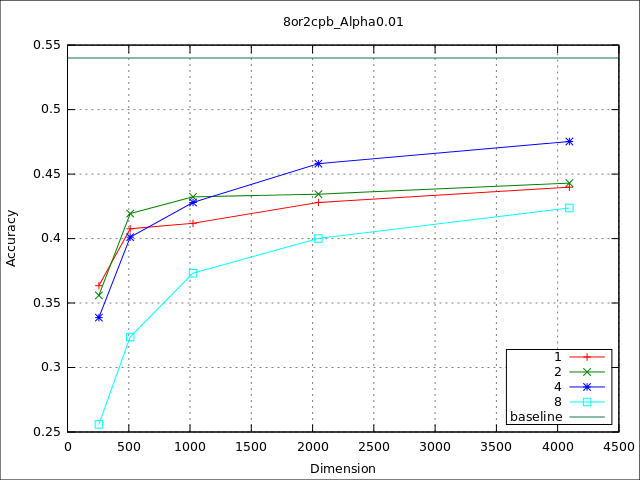
\includegraphics[scale=0.6]{img/resultados/reales/median_8or2cpb_Alpha0,01.png}
				\caption[Reales con umbral mediana]{Resultado de haber usado la mediana para el calculo del umbral. La mejor clasificación se logra con los siguientes parámetros: \textit{alpha:0.01}, \textit{bits por grupo: 4}, \textit{dim del vector: 4096}, \textit{orientaciones: 8}, \textit{celdas por bloque: 4}.}
				\label{fig: Reales-mediana-8or4cpbAlph0.01}
			\end{figure}
			
			\begin{figure}[htbp]
				\centering
				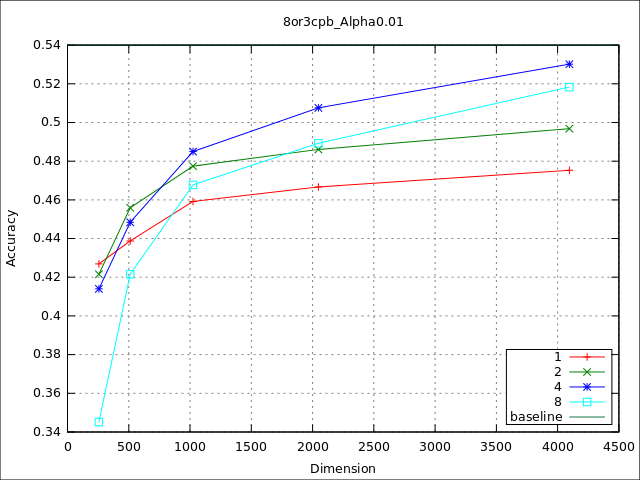
\includegraphics[scale=0.6]{img/resultados/reales/expon_8or3cpb_Alpha0,01.png}
				\caption[Reales con umbral exponencial]{Resultado de haber usado la distribución exponencial para el calculo del umbral. La mejor clasificación se logra con los siguientes parámetros: \textit{alpha:0.01}, \textit{bits por grupo: 4}, \textit{dim del vector: 4096}, \textit{orientaciones: 8}, \textit{celdas por bloque: 9}.}
				\label{fig: Reales-expon-8or9cpbAlph0.01}
			\end{figure}
			
			\begin{figure}[htbp]
				\centering
				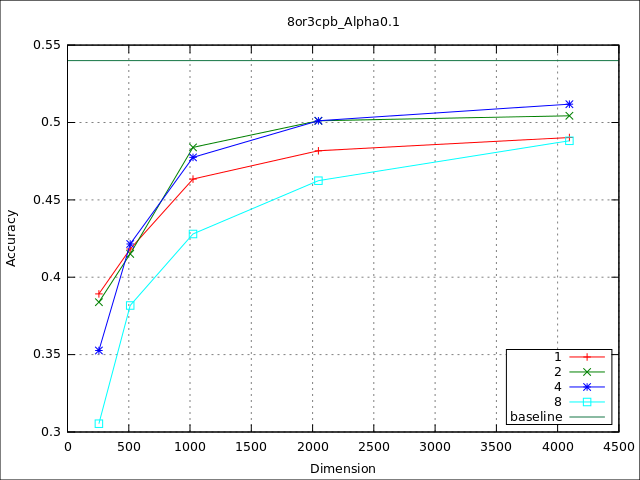
\includegraphics[scale=0.6]{img/resultados/reales/bootstrap_8or3cpb_Alpha0,1.png}
				\caption[Reales con umbral boostrap]{Resultado de haber usado bootstrap para el calculo del umbral. La mejor clasificación se logra con los siguientes parámetros: \textit{alpha:0.1}, \textit{bits por grupo: 4}, \textit{dim del vector: 4096}, \textit{orientaciones: 8}, \textit{celdas por bloque: 9}.}
				\label{fig: Reales-bootstrap-8or9cpbAlph0.1}
			\end{figure}
			
		Después de presentar estos gráficos aclaro que los siguientes experimentos se realizaron utilizando la mejor configuración observada (8 orientaciones, 9 grupos por bloque). Comparación final con los resultados de Wang.
	\begin{table}
		\centering
		\begin{tabular}{ | l | l | l | p{5cm} |}
    			\hline
    				\textbf{NATIVE + FERNS} & \textbf{Score} \\ \hline
    				Wang et al. & 0.54\% \\ \hline
    				Media & 0.53\% \\ \hline
    				Mediana & 0.47\%\\ \hline
    				Exponencial & 0.53\% \\ \hline
    				Bootstrap & 0.51\%\\ 
    			\hline
    		\end{tabular}
    		\caption{Tabla comparativa entre el resultado obtenido por Wang para imágenes naturales y los obtenidos en el presente trabajo, utilizando los cuatro umbrales propuestos.}
    	\end{table}
    	
    	Teniendo en cuenta el resultado de Wang para las imágenes sintéticas, paso a mostrar 
los resultados de haber ido incrementando la proporcion de muestras sintéticas al momento de entrenar al clasificador.

			\begin{figure}[htbp]
				\centering
				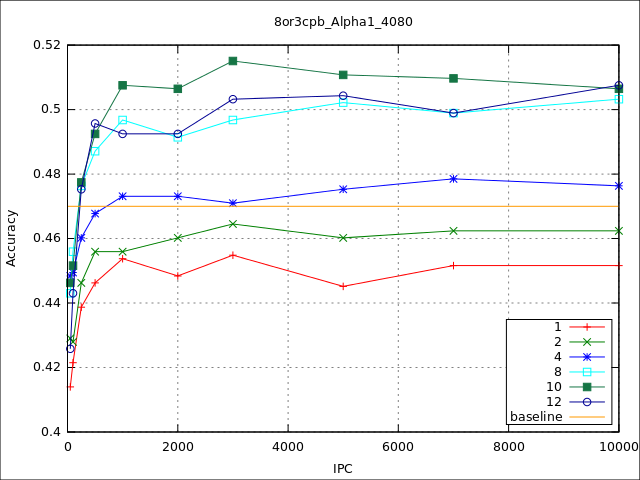
\includegraphics[scale=0.6]{img/resultados/sinteticas/best_media_8or3cpb_Alpha1_4080.png}
				\caption[Sintéticas media bajo resultado]{}
				\label{fig: Sinteticas-media-bajo}
			\end{figure}
			
			\begin{figure}[htbp]
				\centering
				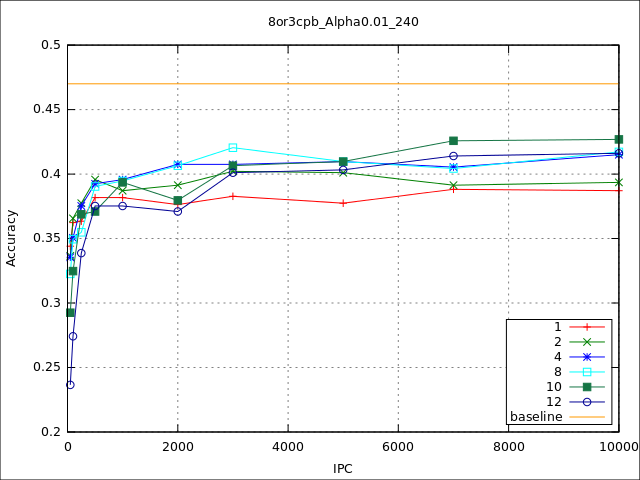
\includegraphics[scale=0.6]{img/resultados/sinteticas/worst_media_8or3cpb_Alpha0,01_240.png}
				\caption[Sintéticas media mejor resultado]{}
				\label{fig: Sinteticas-media-mejor}
			\end{figure}
			
			\begin{figure}[htbp]
				\centering
				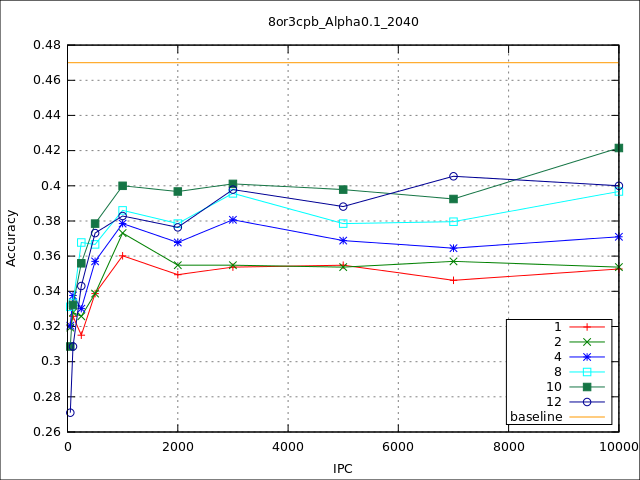
\includegraphics[scale=0.6]{img/resultados/sinteticas/best_median_8or3cpb_Alpha0,1_2040.png}
				\caption[Sintéticas mediana mejor resultado]{}
				\label{fig: Sinteticas-median-mejor}
			\end{figure}
	
			\begin{figure}[htbp]
				\centering
				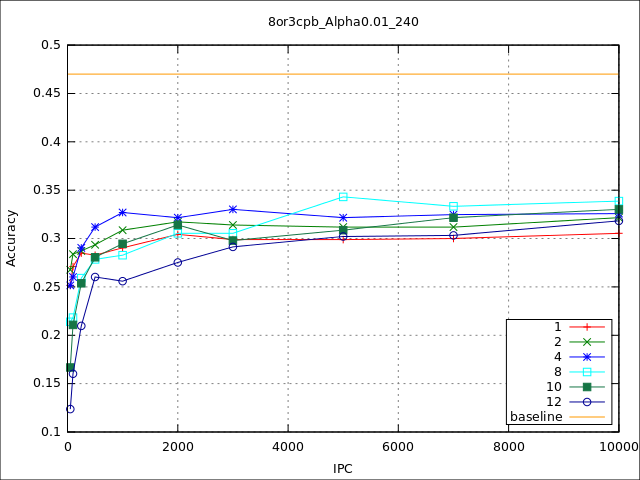
\includegraphics[scale=0.6]{img/resultados/sinteticas/worst_median_8or3cpb_Alpha0,01_240.png}
				\caption[Sintéticas mediana peor resultado]{}
				\label{fig: Sinteticas-median-bajo}
			\end{figure}
				
			\begin{figure}[htbp]
				\centering
				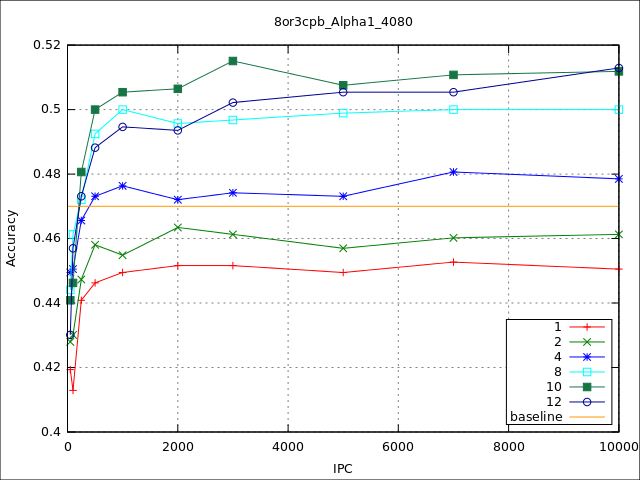
\includegraphics[scale=0.6]{img/resultados/sinteticas/best_expon_8or3cpb_Alpha1_4080.png}
				\caption[Sintéticas exponencial mejor resultado]{}
				\label{fig: Sinteticas-expon-mejor}
			\end{figure}
	
			\begin{figure}[htbp]
				\centering
				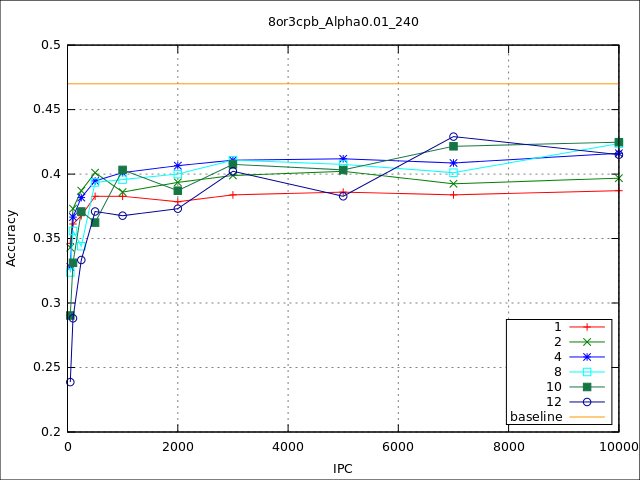
\includegraphics[scale=0.6]{img/resultados/sinteticas/worst_expon_8or3cpb_Alpha0,01_240.png}
				\caption[Sintéticas exponencial peor resultado]{}
				\label{fig: Sinteticas-expon-bajo}
			\end{figure}
			
			\begin{figure}[htbp]
				\centering
				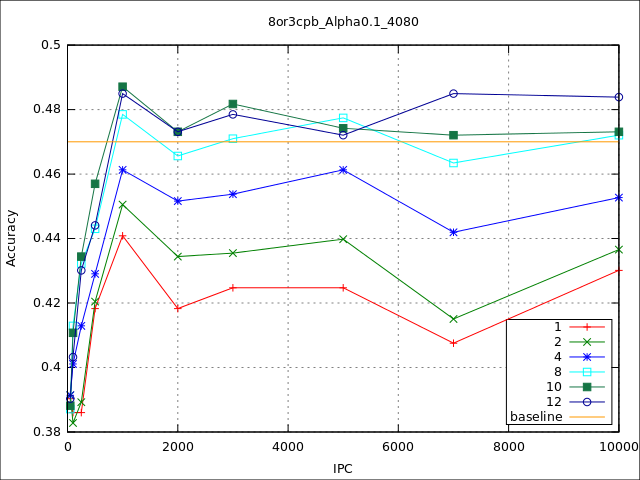
\includegraphics[scale=0.6]{img/resultados/sinteticas/best_bootstrap_8or3cpb_Alpha0,1_4080.png}
				\caption[Sintéticas bootstrap mejor resultado]{}
				\label{fig: Sinteticas-bootstrap-mejor}
			\end{figure}
	
			\begin{figure}[htbp]
				\centering
				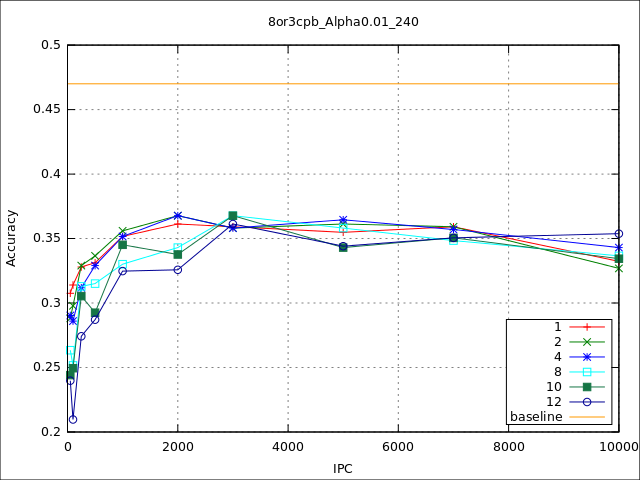
\includegraphics[scale=0.6]{img/resultados/sinteticas/worst_bootstrap_8or3cpb_Alpha0,01_240.png}
				\caption[Sintéticas bootstrap peor resultado]{}
				\label{fig: Sinteticas-bootstrap-bajo}
			\end{figure}

	\newpage
\subsection{Análisis}
	Análisis / discusión
	\begin{itemize}
		\item Comparar la performance al usar diferentes datasets (comparar cantidad de imágenes por clase al usar caracteres sintéticos). Hacer una tabla.
		\item Observaciones sobre errores de clasificación. El problema que surge con algunos caracteres donde no se puede distinguir minúscula de mayúscula con lo cual se producen errores. Mostrar la matriz de confusión del mejor caso donde no se distingan mayúsculas de minúsculas. Otro error donde ciertos caracteres como la "l" se confunden con otros caracteres como el "1".
		\item Comparar en los resultados con los obtenidos por Wang et al. en condiciones similares. Básicamente explicar algo que no explican en su trabajo Wang et al. y que es la influencia en la cantidad de muestras sintéticas por clase.
		\item Análisis de como aumenta la performance de clasificación el mezclar imágenes sintéticas y reales. Mostrar como a medida que aumentamos demasiado la proporción de img. sintéticas, se tiende a disminuir la precisión. Básicamente, la precisión baja para "igualarse" a la precisión obtenida cuando se entrena al clasif con puras imagenes sintéticas (usando la misma cant. de img. por clase).
	\end{itemize}


	%\subsection{Implementación}

	\begin{itemize}
		\item Explicar porque uso python + las librerías involucradas.
		\item Porque uso JSON y no MySQL para almacenar datos.
		\item Datasets usados y su creación.
		\item Pipeline implementado desde la creación del dataset hasta la obtención de resultados del clasificador Random Ferns.
	\end{itemize}

	

